\newcommand{\figuraTensionAguaTemperatura}{%
\begin{figure}[H]
\centering
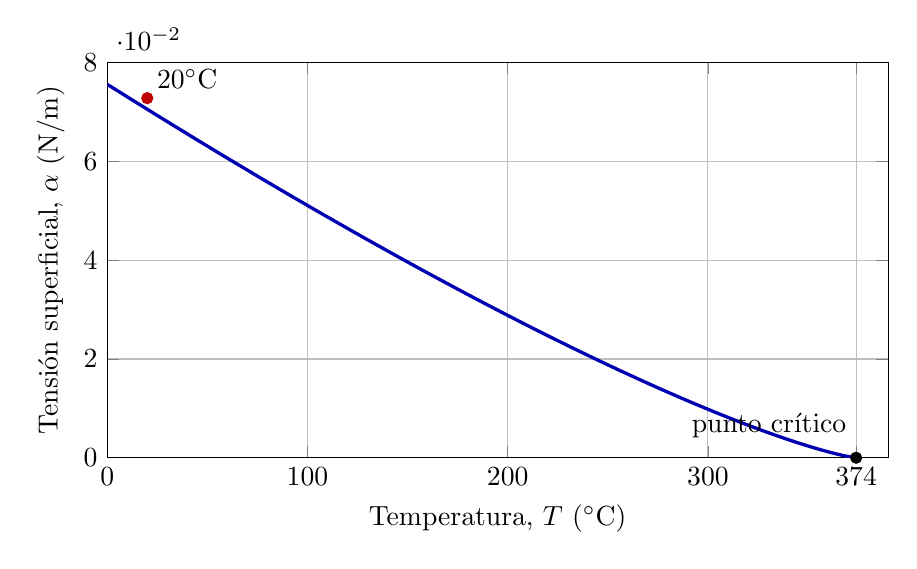
\begin{tikzpicture}
\begin{axis}[
  width=11.5cm,height=6.6cm,
  xlabel={Temperatura, $T\ ({}^\circ\mathrm{C})$},
  ylabel={Tensión superficial, $\alpha\ (\mathrm{N/m})$},
  xmin=0,xmax=390,ymin=0,ymax=0.08,
  xtick={0,100,200,300,374},
  ytick={0,0.02,0.04,0.06,0.08},
  grid=major]
  \addplot[very thick,blue!70!black,domain=0:374,samples=160]
    {0.0756*(1-x/374)^1.26};
  \addplot[only marks,mark=*,red!75!black] coordinates {(20,0.0728)};
  \node[anchor=south west] at (axis cs:20,0.0728) {$20^\circ\mathrm{C}$};
  \addplot[only marks,mark=*,black] coordinates {(374,0)};
  \node[anchor=south east] at (axis cs:374,0.002)
    {punto crítico};
\end{axis}
\end{tikzpicture}
\caption{Disminución aproximada de la tensión superficial de una interfaz
agua--aire limpia con la temperatura. La tensión se anula en el punto crítico.}
\label{fig:tension-agua-temperatura}
\end{figure}%
}